\documentclass{article}
\usepackage{amsmath,amssymb,amsthm,latexsym,paralist,url}
\usepackage[margin=1in]{geometry}
\usepackage{graphicx}
\usepackage{tikz}
\usetikzlibrary{arrows,automata}

\theoremstyle{definition}
\newtheorem{problem}{Problem}
\newtheorem*{solution}{Solution}
\newtheorem*{resources}{Resources}


\newcommand{\honor}{\noindent \textbf{Aggie Honor Statement: }On my honor as an Aggie, I have neither
  given nor received any unauthorized aid on any portion of the academic work included in this assignment.
}

 
\newcommand{\checklist}{\noindent\textbf{Checklist:}
Did you...
\begin{compactenum}
\item abide by the Aggie Honor Code?
\item solve all problems?
\item start a new page for each problem?
\item show your work clearly?
\item type your solution?
\item submit a PDF to eCampus?
\end{compactenum}
}

\newcommand{\problemset}[1]{\begin{center}\textbf{Problem Set #1}\end{center}}
\newcommand{\duedate}[1]{\begin{quote}\textbf{Due: #1} on eCampus (\url{ecampus.tamu.edu}). \\You must show your work in order to recieve credit.\end{quote}}
\newcommand{\mysectionnumber}[0]{503}

\title{CSCE 222: Discrete Structures for Computing\\Section \mysectionnumber\\Fall 2016}
\author{YOUR NAME HERE}

\begin{document}

\maketitle

\problemset{7}

\duedate{16 October 2016 (Sunday) before 11:59 p.m.}

\bigskip

% Languages and Grammars
\begin{problem} (25 points)\\
\begin{enumerate}
\item A \textbf{palindrome} is a string that reads the same backward as it does forward, i.e. a string $w$, where $w=w^R$, where $w^R$ is the reversal of the string $w$.  Give a context-free grammar, expressed in Backus-Naur form, that generates the set of all palindromes over the alphabet $\Sigma=\{a,b,c\}$.
\item Use bottom-up parsing determine whether the following strings belong to $L(G)$, where $G=(\Sigma,N,S,P)$, where $\Sigma=\{a,b,c\}$, $N=\{S,A,B,C\}$, and $P=\{S\to AB,A\to aC,B\to aB, B\to bC, B\to b, C \to cb, C\to b\}$.
\begin{enumerate}
\item abbb
\item ababb
\item acbaacb
\item acbaaabcb
\end{enumerate}
\end{enumerate}
\end{problem}


%\begin{solution}\ \\
%\end{solution}

%\newpage

% Languages and Grammars
\begin{problem} (25 points)\\
In \textbf{extended Backus-Naur form (EBNF)}, the symbol $?$ indicates that the preceding symbol, or group of symbols inside parentheses, is optional (can appear zero or once); the symbol $*$ indicates the the preceding symbol or group can be repeated zero or more times; the symbol $+$ indicates that the preceding symbol or group can appear one or more times.
\begin{enumerate}
\item Describe the language generated by each of these grammars expressed in EBNF.
\begin{enumerate}
\item 
\begin{align*}
S & ::= L\text{+}D\text{?}L\text{+}\\
L & ::= a \mid b \mid c\\
D & ::= 0 \mid 1
\end{align*}
\item 
\begin{align*}
S & ::= PD\text{+} \mid D\text{+}\\
P & ::= + \mid -\\
D & ::= 0 \mid 1 \mid 2 \mid 3 \mid 4 \mid 5 \mid 6 \mid 7 \mid 8 \mid 9\\
\end{align*}
\item 
\begin{align*}
S & ::= L\text{*}(D\text{+})\text{?}L\text{*}\\
L & ::= x \mid y\\
D & ::= 0 \mid 1
\end{align*}
\end{enumerate}
\item Show that EBNF and BNF can generate the same languages by describing how productions for a grammar in EBNF can be translated into a set of productions for the grammar in BNF.
\end{enumerate}
\end{problem}

%\begin{solution}\ \\
%\end{solution}

%\newpage

% Finite State Machines
\begin{problem} (25 points)\\
Construct deterministic finite-state automata that recognize each of these languages.
\begin{enumerate}
\item the set consisting of the bitstrings 00, 11, and 010.
\item the set of bitstrings that start with 10 and end with one or more 1s.
\item the set of bitstrings consisting of an odd number of 0s followed by a final 1.
\item the set of bitstrings that have neither two consecutive 0s nor two consecutive 1s.
\end{enumerate}
\end{problem}

%\begin{solution}\ \\
%\end{solution}

%\newpage

% Finite State Machines
\begin{problem} (25 points)\\
Consider this nondeterministic finite-state automaton:\\

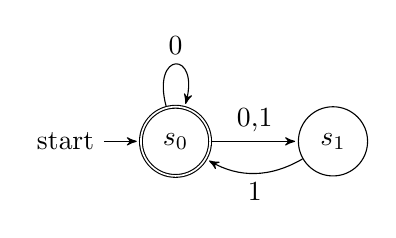
\begin{tikzpicture}[>=stealth',shorten >=1pt,auto,node distance=2cm]
  \node[initial,state,accepting] (S)      {$s_0$};
  \node[state]         (q1) [right of=S]  {$s_1$};

  \path[->] (S)  edge [loop above] node {0} (S)
             edge              node {0,1} (q1)
        (q1) edge [bend left]  node {1} (S);
\end{tikzpicture}

\begin{enumerate}
\item Construct a deterministic finite-state automaton that recognizes the same language.
\item What is the language that the automaton recognizes?
\end{enumerate}
\end{problem}

%\begin{solution}\ \\
%\end{solution}


\bigskip
\honor

\bigskip
\checklist
\end{document}
